\documentclass{article}
\usepackage[slovene]{babel}
\usepackage[utf8]{inputenc}
\usepackage[T1]{fontenc}

\usepackage{amsmath}
\usepackage{amsthm}
\usepackage{amsfonts}
\usepackage{url}
\usepackage{graphicx}
\usepackage{enumerate}
\usepackage{listings}
\graphicspath{ {images/} }

\newtheorem{algoritm}{Algoritem}[section]
\newtheorem{theorem}{Izrek}[section]
\newtheorem{corollary}{Corollary}[theorem]
\newtheorem{lemma}[theorem]{Lema}

\setlength\parindent{0pt}

\begin{document}

\begin{titlepage}
	\centering
	{\scshape\LARGE Fakulteta za matematiko in fiziko \par}
	\vspace{1cm}
	{\scshape\Large Računsko podprto geometrijsko oblikovanje\par}
	\vspace{1.5cm}
	{\huge\bfseries VS postopek za izračun vrednosti polinomov več spremenljivk\par}
	\vspace{2cm}
	{\Large\itshape Janez Radešček, Miha Avsec\par}
	\vfill

	\vfill

% Bottom of the page
	{\large \today\par}
\end{titlepage}


\section{Decasteljou}

Naj bo $T$ trikotnik v ravnini, ter naj bodo $(r,s,t)$ baricentrične koordinate točke $P$ glede na trikotnik $T$. V tem primeru lahko vsak polinom stopnje $d$ definiran nad trikotnikom $T$ zapišemo v Bernsteinovi bazi kot
$$p(r,\\s,\\t) = \sum_{i=0}^{d}\sum_{j=0}^{i}b_{d-i,i-j,j}B_{d-i,i-j,j}^{d},$$
kjer velja
$$B_{i,j,k}^{d}(r,s,t) = \frac{d!}{i!j!k!}rîs^jt^k.$$

Tako podan polinom lahko evaluiramo s pomočjo deCasteljouvovega algoritma
\begin{algoritm}
Naj bo p polinom stopnje $d$ podan v Bezierjevi obliki, ter naj bodo $ r,s,t$ baricentirčne koordinate točke za katere velja $r \geq s,r \geq t$, tedaj lahko s sledečim algoritmom izračunamo vrenost polinoma p v točki $(r,s,t)$
\begin{lstlisting}[escapeinside={(*}{*)}]
for k=1:d
  for i=0:d-k
      for j=0:i
          (*$b_{d-i-k,i-j,j}^k = r*b_{d-i-k+1,i-j,j}^{k-1}+s*b_{d-i-k,i-j+1,j}^{k-1} +r*b_{d-i-k,i-j,j+1}^{k-1}  $*)
(*$p(r,s,t) = b_{0,0,0}^{d}$*)
\end{lstlisting}
\end{algoritm}

Ta algoritem potrebuje $d(d+1)(d+2)/2$ operacij.




\section{Modificirana Bernstein-Bezierjeva reprezentacija}

Če imamo podan polinom v Bernsteinovi obliki $$p(r,\\s,\\t) = \sum_{i=0}^{d}\sum_{j=0}^{i}b_{d-i,i-j,j}B_{d-i,i-j,j}^d(r,\\s,\\t),$$
potem lahko tak polinom enostavno prepišemo v obliko
$$p(r,\\s,\\t) = \sum_{i=0}^{d}\sum_{j=0}^{i}c_{d-i,i-j,j}r^{d-i}s^{i-j}t^j,$$
tako da za koeficiente $c_{d-i,i-j,j}$ vzamemo
$$c_{d-i,i-j,j} = \frac{d!}{(d-i)!(i-j)!j!}b_{d-i,i-j,j}, \quad j=0,\ldots, i;\\ i = 0,\ldots,d.$$
Tej obliki polinoma rečemo modificirana Bernstein-Bezierjeva oblika ali krajše MBB. Pokazati želimo, da se polinom v MBB obliki, da evaluirati hitreje kakor v klasični Bezierjevi obliki. Ideja, ki se skriva v ozadju je ta, da lahko p zapišemo v gnezdeni obliki. Poglejmo si na primeru polinomov stopnje $2$. Označimo kontrolne točke na sledeči način:

\begin{center}
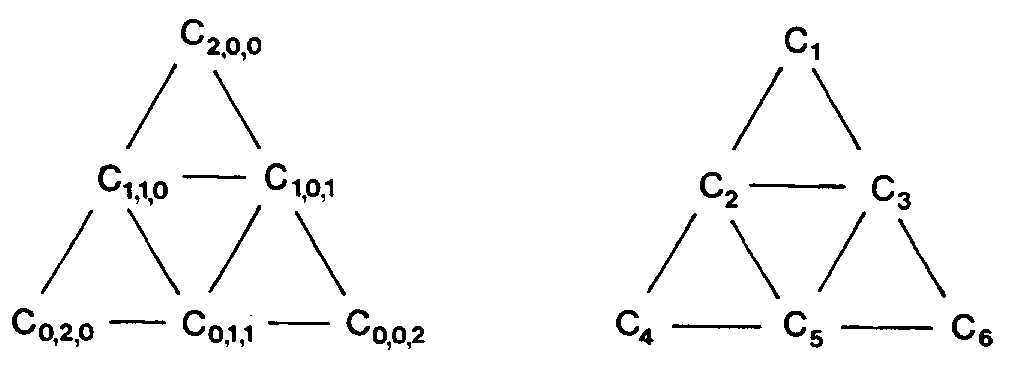
\includegraphics[width=.9\linewidth]{graf.png}
\end{center}

Če razpišemo sedaj polinom glede na spremenljivko $r$ dobimo:

\begin{align}
p(r,s,t) &= \sum_{i=0}^{2}\sum_{j=0}^{i}c_{2-i,i-j,j}r^{2-i}s^{i-j}t^j \nonumber \\ \nonumber
&= r^2\sum_{j=0}^{0}c_{2,-j,j}s^{-j}t^j + r\sum_{j=0}^{1}c_{1,1-j,j}s^{1-j}t^j + \sum_{j=0}^{2}c_{0,2-j,j}s^{2-j}t^j \\ \nonumber
&= r^2(c_1) + r(c_2s+c_3t) + (c_4s^2+c_5st+c_6t^2)\\ \nonumber
&= r^2(c_1+\frac{s}{r}c_2+\frac{t}{r}c_3+\frac{s^2}{r^2}c_4+\frac{st}{r^2}c_5+\frac{t^2}{r^2}c_6) \\ \nonumber
&= r^2(\frac{s}{r}(c_2+\frac{s}{r}c_4+\frac{t}{r}c_5)+\frac{t}{r}(\frac{t}{r}c_6+c_3)+c_1) \nonumber
\end{align}

Tu je potrebno biti pozoren na to, da ne delimo z $0$. Torej je treba ločiti primere glede na to v katerem odseku trikotnika se naše baricentrične koordinate nahajajo in podobno razvijemo po spremenljivki $s$ ali $t$.
V Primeru ko razvijamo po $r$ dobimo algoritem

\begin{algoritm}
Naj bo p polinom stopnje $n$ podan v MBB obliki, ter naj bodo $ r,s,t$ baricentirčne koordinate točke za katere velja $r \geq s,r \geq t$, tedaj lahko s ledečim algoritmom izračunamo vrenost polinoma p v točki $(r,s,t)$
\begin{lstlisting}[escapeinside={(*}{*)}]
sr = s/r,	 tr= s/r
A = (*$c_{0,n,0}$*);
for i = 1:n
    B = (*$c_{0,n-i,i}$*)
    for j = i:-1:1
        B = B*tr + (*$c_{i-j+1,n-i,j-1}$*);
    end
    A = A *sr +B;
end
p(r,s,t) = A(*$r^n$*)
\end{lstlisting}
\end{algoritm}

Zgornji algoritem potrebuje $(n^2+5n)/2$ množenj, $2$ deljenj, ter $n-1$ množenj za izračun $r^n$, kar lahko v splošnem naredimo tudi z manj operacijami (npr. za algoritmom kvadriraj in zmnoži).
Potrebno je povedati še, kako se odločimo katero verzijo algoritma bomo vzeli.

\begin{center}
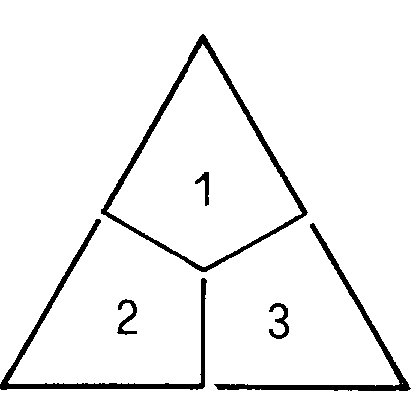
\includegraphics[width=.3\linewidth]{graf1.png}
\end{center}

Zgornji algoritem deluje za regijo ena, v kateri se nahajamo če $r \geq s,r \geq t$. S spremembami po kateri spremenljivki razvijamo pa pokrijemo tudi regiji $2$ in $3$. Pri čemer je regija $2$ določena z $s > r, s \geq t$ in razvijamo po $s$, regija 3 pa z $t > r, t>s$ pri čemer razvijamo po $t$.


\section{Polinom v Taylorjevi vrsti}

Naj bo T trikotnik. Naj bo $p$ polinom stopnje $n$ definiran na $T$. Polinom $p$ lahko zapišemo v Taylorjevi obliki kot 
$$p(u,v) = \sum_{i = 0}^n{\sum_{j=0}^{n-i}{a_{i,j}u^iv^j }}.$$To obliko bomo krajše klicali $TAY$.  Vrednost polinoma $p$ v točki $(u,v)$ lahko izračunamo s sledečim algoritmom.

\begin{algoritm}
\begin{lstlisting}[escapeinside={(*}{*)}]

p = (*$a_{0,n}$*)
for i = 1:d
    A = (*$a_{i,n-i}$*)
    for j = 1:i
        A = A * u + (*$a_{i-j,n-i}$*)
    end
    p = p * v + A
end
\end{lstlisting}
\end{algoritm}

Ta postopek potrebuje $(n^2+3n)/2$ množenj.


\section{Polinomi na tetraedrih}

Naj bo T tetraeder. Za vsako točko $U$ iz $T$ naj bodo $(r,s,t,u)$ pripadajoče Baricentrične koordinate glede na $T$.  Naj bo $p$ polinom stopnje $n$ definiran na $T$. Polinom $p$ lahko zapišemo v modificirani Bernstein-Bezierjevi obliki kot 
$$p(r,s,t,u) = \sum_{i = 0}^n{\sum_{j=0}^{i}{\sum_{k = 0}^{j}{c_{d-i,i-j,j-k,k} r^{d-i} s^{i-j} t^{j-k} u^k}}}.$$

%zavrtimo točke tako da je računanje efficient

Vrednost polinoma $p$ v točki $(r,s,t,u)$ lahko izračunamo s sledečim algoritmom.

\begin{algoritm}
\begin{lstlisting}[escapeinside={(*}{*)}]

TODO

\end{lstlisting}
\end{algoritm}

Ta postopek potrebuje $(n^3+ 6d^2 + 17d)/6$ množenj in 3 deljenja.




\end{document}
